\documentclass[reqno]{amsart}
\usepackage{amscd, amssymb, amsmath, amsthm}
\usepackage{graphicx}
\usepackage[colorlinks=true,linkcolor=blue]{hyperref}
\usepackage[utf8]{inputenc}
\usepackage[T1]{fontenc}
\usepackage{textcomp}
\usepackage{babel}
%% for identity function 1:
\usepackage{bbm}
%%For category theory diagrams:
\usepackage{tikz-cd}

\usepackage[backend=biber]{biblatex}
\addbibresource{notes.bib}


\setlength\parindent{0pt}

\pdfsuppresswarningpagegroup=1

\newtheorem{theorem}{Theorem}[section]
\newtheorem{lemma}[theorem]{Lemma}
\newtheorem{proposition}[theorem]{Proposition}
\newtheorem{corollary}[theorem]{Corollary}
\newtheorem{conjecture}[theorem]{Conjecture}

\theoremstyle{definition}
\newtheorem{definition}[theorem]{Definition}
\newtheorem{example}[theorem]{Example}
\newtheorem{exercise}[theorem]{Exercise}
\newtheorem{problem}[theorem]{Problem}
\newtheorem{question}[theorem]{Question}

\theoremstyle{remark}
\newtheorem*{remark}{Remark}
\newtheorem*{note}{Note}
\newtheorem*{solution}{Solution}



%Inequalities
\newcommand{\cycsum}{\sum_{\mathrm{cyc}}}
\newcommand{\symsum}{\sum_{\mathrm{sym}}}
\newcommand{\cycprod}{\prod_{\mathrm{cyc}}}
\newcommand{\symprod}{\prod_{\mathrm{sym}}}

%Linear Algebra

\DeclareMathOperator{\Span}{span}
\DeclareMathOperator{\im}{im}
\DeclareMathOperator{\diag}{diag}
\DeclareMathOperator{\Ker}{Ker}
\DeclareMathOperator{\ob}{ob}
\DeclareMathOperator{\Hom}{Hom}
\DeclareMathOperator{\Mor}{Mor}
\DeclareMathOperator{\sk}{sk}
\DeclareMathOperator{\Vect}{Vect}
\DeclareMathOperator{\Set}{Set}
\DeclareMathOperator{\Group}{Group}
\DeclareMathOperator{\Ring}{Ring}
\DeclareMathOperator{\Ab}{Ab}
\DeclareMathOperator{\Top}{Top}
\DeclareMathOperator{\hTop}{hTop}
\DeclareMathOperator{\Htpy}{Htpy}
\DeclareMathOperator{\Cat}{Cat}
\DeclareMathOperator{\CAT}{CAT}
\DeclareMathOperator{\Cone}{Cone}
\DeclareMathOperator{\dom}{dom}
\DeclareMathOperator{\cod}{cod}
\DeclareMathOperator{\Aut}{Aut}
\DeclareMathOperator{\Mat}{Mat}
\DeclareMathOperator{\Fin}{Fin}
\DeclareMathOperator{\rel}{rel}
\DeclareMathOperator{\Int}{Int}
\DeclareMathOperator{\sgn}{sgn}
\DeclareMathOperator{\Homeo}{Homeo}
\DeclareMathOperator{\SHomeo}{SHomeo}
\DeclareMathOperator{\PSL}{PSL}
\DeclareMathOperator{\Bil}{Bil}
\DeclareMathOperator{\Sym}{Sym}
\DeclareMathOperator{\Skew}{Skew}
\DeclareMathOperator{\Alt}{Alt}
\DeclareMathOperator{\Quad}{Quad}
\DeclareMathOperator{\Sin}{Sin}
\DeclareMathOperator{\Supp}{Supp}
\DeclareMathOperator{\Char}{char}
\DeclareMathOperator{\Teich}{Teich}
\DeclareMathOperator{\GL}{GL}
\DeclareMathOperator{\tr}{tr}
\DeclareMathOperator{\codim}{codim}
\DeclareMathOperator{\coker}{coker}
\DeclareMathOperator{\corank}{corank}
\DeclareMathOperator{\rank}{rank}
\DeclareMathOperator{\Diff}{Diff}
\DeclareMathOperator{\Bun}{Bun}
\DeclareMathOperator{\Sm}{Sm}
\DeclareMathOperator{\Fr}{Fr}
\DeclareMathOperator{\Cob}{Cob}
\DeclareMathOperator{\Ext}{Ext}
\DeclareMathOperator{\Tor}{Tor}



%Row operations
\newcommand{\elem}[1]{% elementary operations
\xrightarrow{\substack{#1}}%
}

\newcommand{\lelem}[1]{% elementary operations (left alignment)
\xrightarrow{\begin{subarray}{l}#1\end{subarray}}%
}

%SS
\DeclareMathOperator{\supp}{supp}
\DeclareMathOperator{\Var}{Var}

%NT
\DeclareMathOperator{\ord}{ord}

%Alg
\DeclareMathOperator{\Rad}{Rad}
\DeclareMathOperator{\Jac}{Jac}

%Misc
\newcommand{\SL}{{\mathrm{SL}}}
\newcommand{\mobgp}{{\mathrm{PSL}_2(\mathbb{C})}}
\newcommand{\id}{{\mathrm{id}}}
\newcommand{\MCG}{{\mathrm{MCG}}}
\newcommand{\PMCG}{{\mathrm{PMCG}}}
\newcommand{\SMCG}{{\mathrm{SMCG}}}
\newcommand{\ud}{{\mathrm{d}}}
\newcommand{\Vol}{{\mathrm{Vol}}}
\newcommand{\Area}{{\mathrm{Area}}}
\newcommand{\diam}{{\mathrm{diam}}}
\newcommand{\End}{{\mathrm{End}}}


\newcommand{\reg}{{\mathtt{reg}}}
\newcommand{\geo}{{\mathtt{geo}}}

\newcommand{\tori}{{\mathcal{T}}}
\newcommand{\cpn}{{\mathtt{c}}}
\newcommand{\pat}{{\mathtt{p}}}

\let\Cap\undefined
\newcommand{\Cap}{{\mathcal{C}}ap}
\newcommand{\Push}{{\mathcal{P}}ush}
\newcommand{\Forget}{{\mathcal{F}}orget}


\title{Homotopy Theory}

\author{Jonas Trepiakas}
\date{}


\begin{document}
    
\maketitle

For these notes, we will follow \cite{Hatcher}, \cite{Bredon}
and \cite{ORW}.

\section{Cofibrations}
For this section, we will follow chapter VII.1 in \cite{Bredon}.\\
\linebreak
One of the fundamental questions in topology is the
"extension problem". Namely, given a map
$g \colon A \to Y$ defined on a subspace $A$ of $X$, when
can we extend this map to all of $X$.

This cannot always be done - for example, as is the case
with $A = Y = S^{n}$ and $X = D^{n+1}$ choosing the
map to be any degree $-1$ map.\\
\linebreak
\begin{question}
    Is the extension problem a \textit{homotopy-theoretic} problem?
    That is, does the answer depend only on the homotopy
    class of $g$?
\end{question}
The answer is: generally not. 
For example, we can take $X = \left[ 0,1 \right] ,
A = \left\{ 0 \right\} \cup \left\{ \frac{1}{n} \mid 
n=1, 2, \ldots \right\} $ and $Y = CA$, the cone
on $A$. Choosing $g$ to be the inclusion of
$A$ into $Y$, this cannot be extended to $X$ as the
extension would be discontinuous at $\left\{ 0 \right\} $.
However, $g \simeq g'$ with $g'$ being the constant
map of $A$ to the vertex of the cone, and $g'$ easily
extends to $X$ by the constant map.\\
\linebreak
It turns out, however, that under some very mild conditions
on the spaces, the problem becomes homotopy theoretic. 
We will now discuss this.

\begin{definition}[Homotopy extension property]
    Let $\left( X,A \right) $ and $Y $ be given spaces.
    Then $\left( X, A \right) $ is said to have
    the \textit{homotopy extension property} with respect to
    $Y$ if the following diagram can always be completed
    to be commutative.
    \begin{equation*}
    \begin{tikzcd}
        A \times I \cup X \times \left\{ 0 \right\} 
        \ar[r] \ar[d, hookrightarrow] & Y\\
        X \times I \ar[ru, dashed]
    \end{tikzcd}
    \end{equation*}

    One can also depict this by the following diagram:
    \begin{equation*}
    \begin{tikzcd}
        A \times \left\{ 0 \right\} \ar[rr, hookrightarrow]
        \ar[dd, hookrightarrow] 
        & & A \times I \ar[dd, hookrightarrow] \ar[ld] \\
        & Y & \\
        X \times \left\{ 0 \right\} \ar[ru] \ar[rr] && X \times I
        \ar[lu, dashed]
    \end{tikzcd}
    \end{equation*}
\end{definition}

If $\left( X,A \right) $ has the homotopy extension property
with respect to $Y$, then the extensibility of maps
$g \colon A \to Y$ depends only on the homotopy class of
$g$. For suppose $H \colon g \simeq g'$ and $g'$ can be
extended to  $\tilde{g'} \colon X \to Y$, 
then define the map
$A \times I \cup  X \times \left\{ 0 \right\} $ by
$\tilde{g'} \times \left\{ 0 \right\} $ on
$X \times \left\{ 0 \right\} $ and
$H$ on $A \times I$. The homotopy extension property for the
pair $(X,A)$ then guarantees the existence of a map
$G \colon X \times I \to Y$ which equals
$g$ on $A \times \left\{ 1 \right\} $, so
$H \left( -,1 \right) \colon X \to Y$ extends $g$.

\begin{definition}[Cofibration]
    Let $f \colon A \to X$ be a map. Then $f$ is called
    a \textit{cofibration} if one can always fill in the following
    commutative diagram given the solid arrows:
    \begin{equation*}
    \begin{tikzcd}
        A \times \left\{ 0 \right\} \ar[dd, "f \times \id"] 
        \ar[rr]
        & & A\times I \ar[dd, "f \times \id"] \ar[dl] \\
            & Y &\\
        X \times \left\{ 0 \right\} \ar[ru]
        \ar[rr]& & X \times I 
        \ar[lu, dashed]
    \end{tikzcd}
    \end{equation*}
    for \textit{any} space $Y$.
\end{definition}

\begin{note}
    If $f$ is an inclusion, the this is the same
    as the homotopy extension property for all $Y$. That attribute
    is sometimes referred to as the 
    \textit{absolute homotopy extension property}.
\end{note}

\begin{theorem}[]
    For an inclusion $A \subset X$, the following are equivalent:
    \begin{enumerate}
        \item The inclusion map $A \hookrightarrow X$ is a 
            cofibration.
        \item $A \times I \cup  X \times  \left\{ 0 \right\} $ 
            is a retract of $X \times I$.
    \end{enumerate}
\end{theorem}

\begin{proof}
    If the inclusion is a cofibration, then choosing
    $Y = A \times I \cup  X \times \left\{ 0 \right\} $ 
    with all arrows being inclusions in the
    diagram of a cofibration, we obtain a map
    $X \times I \to A \times I \cup  X \times \left\{ 0 \right\} $ 
    which is the identity on
    $A \times I \cup  X \times \left\{ 0 \right\} $.\\
    Conversely, if $A \times I \cup  X \times \left\{ 0 \right\} $ 
    is a retract of $X \times I$, then
    we can always complete the diagram by
    mapping $X \times I \to 
    A \times I \cup  X \times  \left\{ 0 \right\} 
    \to Y$ where the second map
    takes the maps $A \times I \to Y$ and
    $X \times \left\{ 0 \right\} \to Y$ from the diagram.
\end{proof}

\begin{corollary}
    If $A$ is a subcomplex of a CW-complex $X$, then
    the inclusion $A \hookrightarrow X$ is a cofibration.
\end{corollary}

\begin{proof}
    We want to construct a retraction
    $X \times I \to A \times I \cup  X \times \left\{ 0 \right\} $.
    We will do so by constructing a retraction
    $\left( \left( A \cup X^{(r)}  \right)\times I  \right) \cup 
    \left( X \times \left\{ 0 \right\}  \right) 
    \to \left( A \times I \right) \cup \left( X \times 
    \left\{ 0 \right\} \right) $ by induction on $r$.
    If it has been defined on the
    $(r-1)$-skeleton, then extending it over an
    $r$-cell is simply a matter of extending a map
    on $S^{r-1} \times I \cup D^{r} \times \left\{ 0 \right\} $ 
    over $D^{r} \times I$ which can be done
    since the pair
    $\left( D^{r} \times I, S^{r-1} \times I
    \cup D^{r} \times \left\{ 0 \right\} \right) $ is homeomorphic
    to $\left( D^{r} \times I, D^{r}\times \left\{ 0 \right\} 
    \right) $.
    See Figure \ref{fig:DUWUWUJK122-png}

    \begin{figure}[htpb]
        \centering
        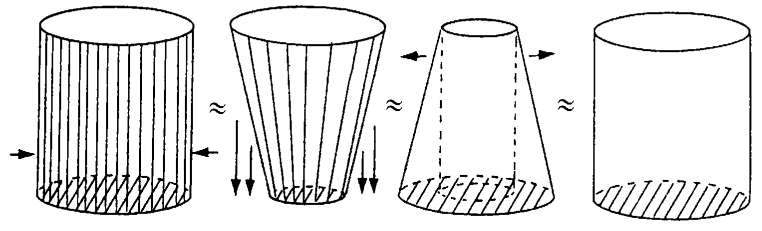
\includegraphics[width=0.8\textwidth]{DUWUWUJK122.png}
        \caption{A homeomorphism of pairs.}
        \label{fig:DUWUWUJK122-png}
    \end{figure}
    These maps for each cell fit together to
    give a map on the $r$-skeleton because of the
    weak topology on $X \times I$. The union of these
    maps for all $r$ gives a map on $X \times I$, again because
    of the weak topology on $X \times I$.
\end{proof}

\begin{theorem}[]
    Assume that $A \subset X$ is closed and that there
    exists a neighborhood $U$ of $A$ and a map
    $\varphi  \colon X \to I$ such that
    \begin{enumerate}
        \item $A = \varphi ^{-1} (0)$.
        \item $\varphi \left( X-U \right) = \left\{ 1 \right\} $.
        \item $U$ deforms to $A$ through $X$ with $A$ fixed.
            That is, there is a map $H \colon U \times I \to X$ 
            such that $H(a,t) = a$ for all $a \in A, H
            (u,0) = 0$, and $H(u,1) \in A$ for all $u \in U$.
    \end{enumerate}
    Then the inclusion
    $A \hookrightarrow X$ is a cofibration. The converse also
    holds.
\end{theorem}

\begin{proof}
    We may assume that $\varphi  = 1$ on a neighborhood
    of $X - U$ by replacing $\varphi $ with
    $\min \left( 2 \varphi , 1 \right) $.
    It suffices to show that there exists a retract
    $\Phi \colon U \times I \to X \times \left\{ 0 \right\} 
    \cup A \times I$ since then the
    map
    \[
    r\left( x,t \right) 
    =
    \begin{cases}
        \Phi\left( x, t \left( 1-\varphi (x) \right)  \right),&
        x \in U\\
        (x,0),& x \not\in U
    \end{cases}
    \] 
    gives a retraction $X \times I \to A \times I \cup 
    X \times \left\{ 0 \right\} $.\\
    We define $\Phi$ by
    \[
    \Phi(u,t) = 
    \begin{cases}
        H\left( u, \frac{t}{\varphi (u)} \right) \times 
        \left\{ 0 \right\},& \varphi (u) > t\\
        H\left( u,1 \right) \times 
        \left\{ t- \varphi (u) \right\} ,& \varphi (u)\le t.
    \end{cases}
    \] 
    The only thing that needs checking here is
    that $\Phi$ is continuous at
    points $\left( u,0 \right) $ such that
    $\varphi (u) = 0$, i.e., points $(a,0)$ for 
    $a \in A$ - indeed here the expression for
    $\varphi (u) > t$ is not defined.

    Recall that a map $f \colon X \to Y$ is continuous
    if for every point $x \in X$ and any neighborhood
    $U$ of $f(x)$, there exists a neighborhood
    $V$ of $x$ such that $f(V) \subset U$.\\
    So let $W$ be a neighborhood of $a = 
    H(a,t)$. Then there exists a neighborhood
    $V \subset W$ containing $a$ such that
    $H\left( V \times I \right) \subset W$, by
    assumption of $H$ being continuous.







\end{proof}


\newpage

\section{Homotopy Groups}

\subsection{Homotopy}
We follow chapter 14 of \cite{Bredon} for this subsection.\\

To start of, we recall the basic definitions of homotopies.

\begin{definition}[Homotopy]
    Two maps $f_0, f_1 \colon X \to Y$ are said to
    be \textit{homotopic} if there exists a homotopy
    $F \colon X \times I \to Y$ such that
    $F(x,0) = f_0(x)$ and $F(x,1) = f_1(x)$ for
    all $x \in X$.
\end{definition}

\begin{definition}[Homotopy equivalence]
    A map $f \colon X \to Y$ is said to be a \textit{homotopy
    equivalence} if it is an isomorphism in
    $\hTop$.
\end{definition}

\begin{lemma}[Reparametrization Lemma]
    Let $\varphi_1, \varphi_2$ be maps
    $\left( I, \partial I \right) \to 
    \left( I, \partial I \right) $ which are equal on
    $\partial I$. Let
    $F \colon X \times I \to Y$ be a homotopy and let
    $G_i (x,t) = F\left( x, \varphi_i(t) \right) $ for
    $i = 1,2$. Then $G_1 \simeq G_2 \rel
    X \times \partial I$.
\end{lemma}

We shall use $c$ to denote the constant homotopy.

\begin{proposition}[]
    $F * c \simeq F \rel X \times \partial I$ and
    $c * F \simeq F \rel X \times \partial I$.
\end{proposition}

\begin{definition}[]
    If $F \colon X \times I \to Y$ is a homotopy, then we
    define $F^{-1} \colon X \times I \to Y$ by
    $F^{-1}\left( x,t \right) = F(x,1-t)$. 
\end{definition}

Note that $F^{-1}$ is precisely the inverse
to $F$ in $\hTop$.

\begin{proposition}[]
    For any homotopies $F,G,H$ for which the
    concatenations 
     are defined, we have
     \[
         \left( F * G  \right) * H
         \simeq F * \left( G * H \right) 
         \rel X \times \partial I.
     \] 
\end{proposition}


\begin{proposition}[]
    For homotopies $F_1, F_2, G_1, G_2$,
    if $F_1 \simeq F_2 \rel X \times \partial I$ and
    $G_1 \simeq G_2 \rel X \times \partial I$, then
    $F_1 * G_1 \simeq F_2 * G_2 \rel X \times \partial I$.
\end{proposition}

Note that all of the discussion of concatenation of
homotopies goes through with no difficulties for the cases
in which all homotopies are relative to some subspace
$A \subset X$ or are homotopies of pairs
$\left( X, A  \right) \to \left( Y, B \right) $.\\
It follows that homotopy between maps of
pairs $\left( X,A \right) \to \left( Y,B \right) $ is
an equivalence relation. The set of homotopy classes
of these maps is commonly denoted by
$\left[ X,A ; Y ,B \right] $ or just
$\left[ X;Y \right] $ if $A = \varnothing$.

\begin{theorem}[]\label{Thm:299221}
    If $f_0 \simeq f_1 \colon X \to Y$ then
    $M_{f_0} \simeq M_{f_1} \rel
    X + Y$ and
    $C_{f_0} \simeq C_{f_1} \rel
    Y + \text{vertex}$.
\end{theorem}


To show this, one needs the following basic topological
proposition:
\begin{proposition}[] \label{prop:92031999}
    If $f \colon X \to Y$ is a quotient map and
    $K$ is locally compact Hausdorff, then
    $f \times 1 \colon X \times K \to Y \times K$ is
    a quotient map.
\end{proposition}

\begin{proof}[Proof of Theorem \ref{Thm:299221}]
    First, let $F \colon X \times I \to Y$ be the homotopy
    between $f_0$ and $f_1$. Now define $h \colon
    M_{f_0} \to M_{f_1}$ by $h(y) = y$ for
    $y \in Y$ and
    \[
    h\left( x,t \right) = 
    \begin{cases}
        F\left( x,2t \right) ,& t\le \frac{1}{2}\\
        (x, 2t-1),& \frac{1}{2} \le t.
    \end{cases}
    \] 
    Define
    $k \colon M_{f_1} \to M_{f_0}$ likewise by
    the identity on $Y$ nad
    \[
    k\left( x,t \right) =
    \begin{cases}
        F^{-1}\left( x,2t \right) ,& t\le \frac{1}{2}\\
        (x,2t-1),& \frac{1}{2}\le t
    \end{cases}.
    \] 
    Then the composition
    $kh \colon M_{f_0} \to M_{f_1}$ is the identity
    on $Y$ and 
    $F * \left( F^{-1} * E \right) $ on
    the cylinder portion, where $E \colon X \times I \to 
    M_{f_0}$ is induced by the identity on
    $X \times I \to X \times I$.
    This is homotopic to the identity 
    $\rel X \times \left\{ 1 \right\} + Y$.
    Similarly for $hk$.
    In now remains to check the continuity of this homotopy.
    We have a homotopy $M_{f_0} \times I \to 
    M_{f_0}$. We now claim that
    $M_{f_0} \times I \cong M_{f_0 \times I}$. Indeed
    then, using that
    $M_{f_0 \times I} = 
    \frac{X \times I \times I \sqcup Y \times I}{
    \left( (x,0,k) \sim (f_0(x),k \right) }$, it suffices
    to show continuity of the composition
    $X \times I \times I \sqcup Y \times I
    \to M_{f_0} \times I \to M_{f_0}$. 
    For on $Y \times I$, it is the constant homotopy and
    on $X \times I \times I$ it is
    $F * \left( F^{-1} * E \right) \simeq E
    \rel X \times \partial I$. 
    Now, that $M _{f_0} \times I
    \cong M_{f_0 \times I}$ follows from
    Proposition \ref{prop:92031999}.

\end{proof}

Let $f \colon X \to Y$. If $\varphi  \colon Y \to Y'$ is a map,
then there is the induced map
$F \colon M_{f} \to M_{\varphi \circ f}$ induced from
$\varphi $ on $Y$ and the identity on $X \times I$.

\begin{theorem}[]
    If $\varphi  \colon Y \to Y'$ is a homotopy equivalence
    then so is 
    $F \colon \left( M_f , X \right) \to 
    \left( M_{\varphi  \circ f}, X \right) $ and hence
    so is $F \colon C_f \to C_{\varphi  \circ f}$.
\end{theorem}

\begin{proof}
    Let $\psi  \colon Y' \to Y$ be a homotopy inverse
    of $\varphi $ and let $G \colon 
    M_{\varphi \circ f} \to M_{\psi \circ
    \varphi \circ f}$ be the map induced by
    $\psi $ on $Y'$ and the identity on $X \times I$.
    The composition $GF \colon M_f \to M_{\psi \circ \varphi 
    \circ f}$ is induced from $\psi \circ \varphi \colon
    Y \to Y$ and the identity on $X \times I$.
    Let $H \colon Y \times I \to Y$ be a homotopy from
    $\id$ to $\psi \circ \varphi $ ; i.e.,
    $H(y,0) = y$ and $H(y,1) = 
    \psi \varphi (y)$. 
    By the proof of Theorem \ref{Thm:299221}, there is a
    homotopy equivalence
    $h \colon M_f \to M_{\psi \circ \varphi \circ f}\rel X$ given
    by $h(y) = y$ and
     \[
    h(x,t) = 
    \begin{cases}
        H\left( f(x), 2t \right) ,& t\le \frac{1}{2}\\
        (x,2t-1),& t\ge \frac{1}{2}
    \end{cases}.
    \] 
    We claim that
    $h \simeq GF \rel X$. Indeed, the homotopy $H$ can
    be extended to 
    $M_f \times I \to M_{\psi \circ \varphi \circ f}$ by
    putting
    \[
    H\left( (x,s),t \right) 
    =
    \begin{cases}
        H\left( f(x), 2s+t \right) ,& 2s+t \le 1\\
        \left( x, \frac{2s+t-1}{t+1} \right) ,& 2s+t\ge 1
    \end{cases}.
    \] 

    Then $H\left( -,0 \right) = h$ and
    $H\left( -,1 \right) = GF$, so
    since $GF$ is a homotopy equvalence, so is
    $h$.
    Define $F' \colon
    M_{\psi \circ \varphi \circ f} \to 
    M_{\varphi \circ \psi \circ \varphi \circ f}$ 
    as the induced map on mapping cones
    with $\varphi $ on $Y$ and
    the identity on $X \times I$. Then similarly,
    $F' G$ is a homotopy equivalence.\\
    If $k$ is a homotopy inverse of $GF$ then
    $GF k \simeq \id$. If
    $k'$ is a homotopy inverse of $F'G$ then
    $k' F' G \simeq \id$. Thus $G$ has a right
    and left homotopy inverse: $R = Fk$ and
    $L = k'F'$. Then
    $R = \id \circ R \simeq 
    \left( LG \right) R =
    L \left( GR \right) \simeq L \circ \id = L$, so
    $R \simeq L$. That is, 
    $G$ has a homotopy inverse. Therefore,
    $G$ is a homotopy equivalence. Since $G$ and $GF$ are
    homotopy equivalences, so is $F$.
\end{proof}


\begin{problem}[]
    \cite[Ex 14.1]{Bredon} Let $S^2 \cup A$ denote the
    union of the unit $2$-sphere and the line segment
    joining the north and south poles. Show that
    $S^2 \vee S^{1} \simeq
    S^2 \cup A$.
\end{problem}

\begin{proof}
    Define two maps
    $f_0,f_1 \colon \left\{ 0,1 \right\}  \to 
    S^2$ where
    $f_0 (t) = \left( \cos (2\pi t), \sin(2\pi t), 0 \right) $ 
    and $f_1$ is the constant map at $(1,0,0)$. Then
    $f_0 \simeq f_1$, so $C_{f_0} \simeq C_{f_1}$. Now,
    $C_{f_0} = S^2 \cup  A$ while
    $C_{f_1} = S^2 \vee S^{1}$.
\end{proof}

\begin{problem}[]
    \cite[Ex 14.2]{Bredon} 
    Show that the union of a $2$-sphere and a flat
    unit  $2$-cell through the origin is homotopically
    equivalent to the one-point union of two $2$-spheres.
\end{problem}

\begin{proof}
    A $2$-cell is contractible, an
    a $2$-sphere with a $2$-cell inside it is precisely the
    cone of the map
    $S^1 \sqcup S^1 \to S^1$ with the identity on both.
    By \cite[Thm 14.19]{Bredon},
    this is homotopy equivalent to the cone on
    $S^1 \sqcup S^1 \to \left\{ * \right\} $ which is
    $S^2 \vee S^2$.
\end{proof}

\begin{problem}[]
    Show that the union of a standard $2$-torus with two disks,
    one spanning a latitudinal circle and the
    other spanning a longitudinal circle of the torus, is
    homotopically equivalent to a $2$-sphere.
\end{problem}

\begin{proof}
     Using the identification of the torus as the
     quotient space of $I^2$ in the usual way, we can choose
     on spanning circle to be a $2$-cell attached
     along $\left\{ 0 \right\} \times I$ and the
     other to be a $2$-cell attached along
     $I \times \left\{ 0 \right\} $. These are contractible, 
     and the quotient space becomes a $2$-sphere.
\end{proof}


\subsection{Homotopy Groups}

Recall that $\left[ X,A ; Y ,B \right] $ denotes the
set of homotopy classes of maps $X \to Y$ carrying $A$ into
$B$ such that $A$ goes into $B$ during the entire homotopy.

To make a group then, we can select a point $y_0 \in Y$ and
consider the set
\[
\left[ X \times I, X \times \partial I ;
Y , \left\{ y_0 \right\} \right] 
\] 
In this case, the operation of concatenation of homotopies
makes this set into a group.
It is technically also better to choose a basepoint 
$x_0 \in X$ and consider
\[
\left[ X \times I, \left\{ x_0 \right\} \times I
\cup X \times \partial I ; Y , \left\{ y_0 \right\} \right] .
\] 

For the moment, let us set
$A = \left\{ x_0 \right\} \times I \cup 
X \times \partial I$. Then maps
$X \times I \to Y$ which carry $A$ into $\left\{ y_0 \right\} $ 
are in bijective correspondence with maps 
$\left( X \times I \right) / A \to Y$ which take
 the point $\left\{ A \right\} $ into 
 $\left\{ y_0 \right\} $. 
 
 \begin{definition}[Reduced Suspension]
     We define the \textit{reduced suspension} of
     $X$ to be
     \[
     SX = (X \times I) / A =
     \left( X \times I \right) /
     \left( \left\{ x_0 \right\} \times I
     \cup X \times \partial I \right) 
     \] 
 \end{definition}

 The set of homotopy classes of pointed maps
 of a pointed space $X$ to a pointed space $Y$ with
 homotopies preserving the base points will
 be denoted by $\left[ X;Y \right]_* $. 

 Thus
 $\left[ SX;Y \right]_* $ is in canonical bijective
 correspondence with
 $\left[ X \times I, A ; Y , \left\{ y_0 \right\}  \right] $.


 Now, suppose we have pointed maps
 $f,g \colon SX \to Y$. Then they
 induce homotopies
 $f',g' \colon X \times I \to Y$ by precomposing with the
 quotient map
  $X\times I \to SX$. We can then define
  $f' * g' \colon X \times I \to Y$ as usual.
  The resulting pointed map
  $SX \to Y$ will be denoted $f * g$.
  Geometrically, $f * g$ is obtained by
  putting $f$ on the bottom and $g$ on the top
  of the one-point union $SX \vee SX$ and composing
  the resulting map $SX \vee SX \to Y$ with the
  map $SX \to SX \vee SX$ obtained by collapsing the
  middle parameter value $\frac{1}{2}$ copy of
  $X$ in $SX$ to the base point.
  
  \begin{figure}[htpb]
      \centering
      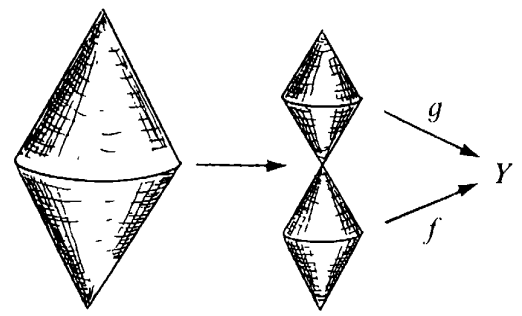
\includegraphics[width=0.6\textwidth]{TKISO0932.png}
      \caption{The product of two map classes
      $SX \to Y$.}
      \label{fig:TKISO0932-png}
  \end{figure}


  For a map $f \colon \left( SX, \left\{ A \right\}  \right) 
  \to \left( Y, \left\{ y_0 \right\}  \right) $, we denote its
  homotopy class in
  $\left[ SX; Y \right]_{*}$ by
  $\left[ f \right] $, and we define
  \[
  \left[ f \right] \left[ g \right] =
  \left[ f*g\right] 
  \] 
  Under this operation, the set
  $\left[ SX;Y \right]_*$ becomes a group.

  \begin{proposition}[]
      The reduced suspension gives
      $S S^{n-1}\cong S^{n}$.
  \end{proposition}

  Thus, we can define $S^{n}$ as the $n$-fold reduced
  suspension of $S^{0}$. As a special case,
  the set $\left[ S^{n};Y \right]_*$ then becomes
  a group for $n>0$. 

  \begin{definition}[$n$ th homotopy group]
      We define
      \[
      \pi_n \left( Y, y_0 \right) =
      \left[ S^{n}; Y \right]_*
      \] 
      with this operation.
  \end{definition}

  \subsubsection{A different way of defining
  $\pi_n \left( Y, y_0 \right) $}
  Note that reduced suspension supplies a parameter in
  $\left[ 0,1 \right] $ and the space
  $S^{n}$ as constructed is the quotient space of
  $I^{n}$ obtained by collapsing the boundary of the cube to a
  point.
  Pointed maps $S^{n}\to Y$ are in bijective correspondence
  with maps $I^{n}\to Y$ taking $\partial I^{n}$ to
  the base point of $Y$. This is a more traditional way
  of defining $\pi_n(Y)$. This becomes the group
  of homotopy classes of maps
  $\left( I^{n},\partial I^{n} \right) \to 
  \left( Y, \left\{ y_0 \right\}  \right) $ with the
  operation being
  \[
  f*g \left( t_1, \ldots, t_n \right) =
  \begin{cases}
      f\left( 2t_1, t_2, \ldots, t_n \right) ,& t_1 \in 
      \left[ 0,\frac{1}{2} \right] \\
      g\left( 2t_1-1, t_2, \ldots, t_n \right) ,& t_1 \in 
      \left[ \frac{1}{2},1 \right] 
  \end{cases}.
  \] 

  \begin{proposition}[]
      For $n\ge 2$, $\pi_n\left( X, x_0 \right)$ is abelian.
  \end{proposition}

  \begin{proof}
      Consider the homotopy in Figure \ref{fig:JIDWOOL0290L-png}.
      We begin by shrinking the domains of $f$ and $g$ to smaller
      subcubes of $I^{n}$, where the region outside is
      mapped to the basepoint. This allows us to move the boxes
      around in a continuous manner. The rest is clear.
      \begin{figure}[htpb]
          \centering
          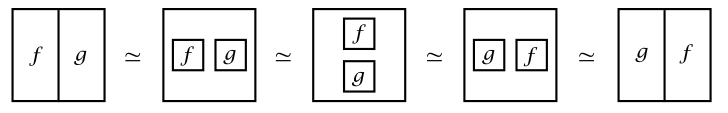
\includegraphics[width=0.8\textwidth]{JIDWOOL0290L.png}
          \caption{The homotopy in question}
          \label{fig:JIDWOOL0290L-png}
      \end{figure}
  \end{proof}

  Next, we want to show that following:
  \begin{proposition}[]\label{Prop:SwjiaKKDNW1102}
      If $X$ is path-connected, then
      $\pi_n\left( X, x_0 \right) \cong
      \pi_n (X, x_1)$ for any two $x_0,x_1 \in X$.
  \end{proposition}

  For this, we introduce an action of
  $\pi_1$ on $\pi_n$.

  \begin{definition}[The action of $\pi_1$ on $\pi_n$]
      Given a path
      $\gamma \colon I \to X$ from
      $x_0$ to $x_1$, we associate to a map
      $f \colon \left( I^{n}, \partial I^{n} \right) \to 
      \left( X, x_1 \right) $ the map
      $\gamma f \colon \left( I^{n}, \partial I^{n} \right) 
      \to \left( X,x_0 \right) $ by shrinking the domain
      of $f$ to a smaller concentric cube in $I^{n}$, then
      inserting the path $\gamma$ on each radial segment
      in the shell between this smaller cube and $\partial
      I^{n}$.
      See Figure \ref{fig:JDWIXHHX011SJ-png}

      \begin{figure}[htpb]
          \centering
          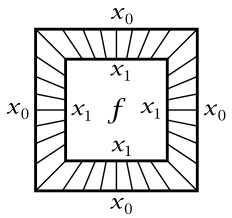
\includegraphics[width=0.25\textwidth]{JDWIXHHX011SJ.png}
          \caption{Depiction of $\gamma f$.}
          \label{fig:JDWIXHHX011SJ-png}
      \end{figure}

  \begin{note}
      We have the following properties
      \begin{enumerate}
          \item $\gamma \left( f+ g \right) 
              \simeq \gamma f + \gamma g$.
          \item $\left( \gamma \eta \right) f \simeq
              \gamma \left( \eta f \right) $.
          \item $\id f \simeq f$, where
              $\id$ denotes the constant path.
      \end{enumerate}

      To see $(1)$, first deform $f$ and $g$ to be
      constant on the right and left halves of
      $I^{n}$, respectively, producing maps
      which we may call $f+0$ and $0+g$, then we 
      can excise a progressively wider symmetric middle slab
      of $\gamma (f+0) + \gamma(0+g)$ (which can be
      seen on the left in Figure \ref{fig:WIWIWSSK11-png})
      until it becomes $\gamma \left( f+g \right) $ (shown on the
      right).

      \begin{figure}[htpb]
          \centering
          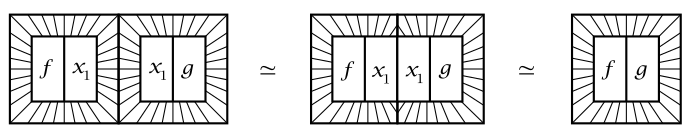
\includegraphics[width=0.8\textwidth]{WIWIWSSK11.png}
          \caption{}
          \label{fig:WIWIWSSK11-png}
      \end{figure}
  \end{note}

  Now if $\beta_{\gamma} \colon \pi_n(X,x_1) \to 
  \pi_n(X, x_0)$ is the change-of-basepoint transformation,
   $\beta_{\gamma}\left[ f \right] =
   \left[ \gamma f \right] $, then
   the above note shows that $\beta_\gamma$ is a group isomorphism.
   This proves Proposition \ref{Prop:SwjiaKKDNW1102}. 
   If we restrict attention to loops
   $\gamma$ at $x_0$, then since $\beta_{\gamma \eta}=
   \beta_{\gamma} \beta_{\eta}$, the map
   $\left[ \gamma \right] \mapsto \beta_{\gamma}$ 
   defines a homomorphism from
   $\pi_1\left( X, x_0 \right) $ to
   $\Aut \left( \pi_n \left( X,x_0 \right)  \right) $ 
   called the \textit{action of $\pi_1$ on $\pi_n$ }.
  \end{definition}

  \begin{note}
  For $n>1$, this action makes
  $\pi_n(X,x_0)$ into a module over the group ring
  $\mathbb{Z}\left[ \pi_1 \left( X,x_0 \right)  \right] $.
  \end{note}  

  \begin{definition}[Simple/abelian spaces]
      A space with trivial $\pi_1$ action on $\pi_n$ is called
      '$n$-simple', and 'simple' means
      ' $n$-simple for all $n$ '. We call
      a space \textit{abelian} if it has
      trivial action of $\pi_1$ on all homotopy groups
      $\pi_n$.
  \end{definition}

  \begin{proposition}[$\pi_n$ is a functor]
      A map $\varphi  \colon \left( X, x_0 \right) \to 
      \left( Y, y_0 \right) $ induces a map
      $\varphi_* \colon \pi_n \left( X, x_0 \right) \to 
      \pi_n \left( Y, y_0 \right) $ defined by
      $\varphi_* \left[ f \right] = \left[ \varphi  f \right] $.
      It is immediate from the definitions that
      $\varphi_*$ is well-defined and a homomorphism
      for $n\ge 1$. The functorial properties are also clear.
  \end{proposition}

  \begin{corollary}
      Homotopy equivalent spaces have isomorphic
      homotopy groups.
  \end{corollary}

  \begin{proposition}[]
      A covering space projection
      $p \colon \left( \tilde{X}, \tilde{x}_0 \right) \to 
      \left( X, x_0 \right) $ induces isomorphisms
      $p_* \colon \pi_n \left( \tilde{X}, \tilde{x}_0 \right) 
      \to \pi_n \left( X, x_0 \right) $ for all
      $n \ge 2$.
  \end{proposition}

  \begin{proof}
      Since 
      $S^{n}$ is path-connected and locally path-connected,
      and simply connected for $n\ge 2$, we find that
      any map
      $\left( S^{n},s_0 \right) 
      \to \left( X, x_0 \right) $ lifts to a 
      map $\left( S^{n},s_0 \right) \to 
      \left( \tilde{X},\tilde{x}_0 \right) $ when
      $n\ge 2$. This gives surjectivity of
      $p_*$.
      For injectivity, suppose
      $p_* \left[ f \right] = \left[ 0 \right] $ where
      $f \colon \left( S^{n}, s_0 \right) \to 
      \left( \tilde{X},\tilde{x}_0 \right) $.
      Let $c_{\tilde{x}_0}$ be the constant map at
      $\tilde{x}_0$. Then
      $p_* \left[ \tilde{x}_0 \right] =
      \left[ 0 \right] $, so by uniqueness of the
      lifting theorem, 
      $\left[ f \right] = \left[ c_{\tilde{x}_0} \right] =
      \left[ 0 \right] $.
  \end{proof}

  \begin{definition}[Aspherical]
      Spaces with $\pi_n = 0$ for all
      $n\ge 2$ are called \textit{aspherical}.
  \end{definition}

  \begin{corollary}
      $S^{1}, T^{n}$ and $K$ are aspherical since
      they have contractible covering spaces.
  \end{corollary}


  \begin{proposition}[]
      \[
      \pi_n \left( \prod_{\alpha} X_{\alpha} \right) 
      \cong \prod_{\alpha} \pi_n \left( X_{\alpha} \right) 
      \] 
  \end{proposition}

  Next we define relative homotopy groups.

  \begin{definition}[Relative homotopy groups]
      Regard $I^{n-1}$ as a face of $I^{n}$ with the last
      coordinate $s_n = 0$ and let
      $J^{n-1}$ be the closure of
      $\partial I^{n}- I^{n-1}$. Then
      we define 
      \[
      \pi_n \left( X, A, x_0 \right) 
      := \left[ I^{n},\partial I^{n}, J^{n-1};
      X , A , x_0\right] 
      \] 
      We shall leave $\pi_0 \left( X, A, x_0 \right) $ undefined
      for now.
  \end{definition}

  We can define a sum operation on $\pi_n \left( X, A, x_0 \right) $ 
  in the same way as for $\pi_n \left( X, x_0 \right) $, except
  now the coordinate $s_n$ now must remain free, so
  we must use one of the other coordinates. Thus
  we must have at least one other coordinate to define
  the same operation. So $\pi_n \left( X, A, x_0 \right) $ is
  a group for $n\ge 2$, and it is abelian for
  $n\ge 3$. For $n=1$, we have
  $I^{1} = \left[ 0,1 \right] , I^{0} = \left\{ 0 \right\} $ 
  and $J^{0} = \left\{ 1 \right\} $, so
  $\pi_1 \left( X, A, x_0 \right) 
  = \left[ I, \left\{ 0 \right\} , \left\{ 1 \right\} ;
  X, A, x_0 \right] $ is the set of homotopy classes of paths in
  $X$ from a varying point in $A$ to the fixed basepoint
  $x_0 \in A$. In general, this is not a group in any
  natural way. \\
  \linebreak
  Now, we saw before that
  $\pi_n \left( X, x_0 \right) $ can be regarded as
  homotopy classes of maps $\left( S^{n}, x_0 \right) \to 
  \left( X, x_0 \right) $. Similarly, collapsing
  $J^{n-1}$ to a point, converts
  $\left( I^{n} , \partial I^{n}, J^{n-1} \right) $ 
  to $\left( D^{n}, S^{n-1}, s_0 \right) $.
  In this case, addition is done by
  the map $c \colon D^{n} \to D^{n} \vee D^{n}$ collapsing
  $D^{n-1} \subset D^{n}$ to a point.


  \subsection{Problem Set 1}

\subsubsection{Exercises}


\begin{exercise}[The action of the fundamental gorup, part
    2]
    Let $X$ be a path-connected, semi-locally simply-connected
    space with basepoint $x$ and $p \colon \tilde{X}\to X$ its
    universal cover. Show that for $n\ge 2$ and
     $\tilde{x} \in X$ with $p (\tilde{x}) = x$, the isomorphism
     $p_* = \pi_n (p) \colon \pi_n \left( \tilde{X}, \tilde{x} \right) 
     \cong \pi_n(X, x)$ allows us to identify the
     action of $\pi_1 \left( X, x \right) $ on $\pi_n (X, x)$ with
     the action of $\pi_1 \left( X, x \right) $ on
     $\pi_n \left( \tilde{X}, \tilde{x} \right) $ induced by
     the group of deck transformations, i.e., the natural action
     of $\pi_1 (X, x)$ on $\tilde{X}$. In particular, make the
     statement precise.
\end{exercise}

\begin{proof}
    We want to show that for $\left[ \gamma \right] 
    \in \pi_1(X, x)$ and
    $\left[ f \right] \in \pi_n \left( X, x \right) $,
    if $\tilde{g}$ is the lift for $\gamma$ starting at
    $\tilde{x}_0$, and
    $\tilde{f} \colon \left( S^{n}, s_0 \right) 
    \to \left( \tilde{X}, \tilde{x}_0 \right) $ is the
    lift of $f$, then
    $p_* \left( \tilde{\gamma} \tilde{f} \right) 
    = \gamma f$. But this follows directly from how
    $\tilde{\gamma} \tilde{f}$ and 
    $\gamma f$ we constructed. Namely, applying
    $p$ to the square used in the definition, we see that we
    obtain $\gamma f$ from $\tilde{\gamma} \tilde{f}$ since
    $p \circ \tilde{\gamma} = \gamma$ and
    $p \circ \tilde{f} = f$.

\end{proof}


\begin{exercise}[]
    Let $X$ and $Y$ be pointed spaces and $n \ge 2$. Show that the
    inclusion $X \vee Y \hookrightarrow X \times Y$ induces
    a surjection $\pi_n \left( X \vee Y \right) 
    \to \pi_n \left( X \times Y \right) $ for all $n$. Furthermore,
    this exhibits $\pi_n \left( X \times Y \right) $ as
    a retract of $\pi_n \left( X \vee Y \right) $ for all $n$.
    (Is this also true for $n=1$?)
\end{exercise}

\begin{proof}
    a
\end{proof}






\subsubsection{Problems}

\begin{problem}[]\label{pset1-degree}
        Fix an isomorphism $H_n\left( S^{n} \right) \cong \mathbb{Z}$.
        We define the degree $\deg f$ of a map
        $f \colon S^{n} \to S^{n}$ to be the integer such that
        $f_* \colon H_n(S^{n}) \to H_n(S^{n})$ sends $1$ to
        $\deg f \in \mathbb{Z}$.
        \begin{enumerate}
            \item Show that taking the degree of a map
                $S^{n} \to S^{n}$ induces a well-defined
                map
                \[
                \deg \colon \pi_n(S^{n}) \to \mathbb{Z}
                \] 
            \item Show that $\deg $ is a group homomorphism.
            \item Show that the map $\deg$ is surjective.
            \item Suppose that $n\ge 2$. Show that
                $\pi_n\left( S^{n} \right) \cong
                \mathbb{Z} \times A$ for some abelian group $A$.
        \end{enumerate}
    \end{problem}

        \begin{proof}


        \begin{enumerate}
            \item Let
                $ \left[ f \right] 
                \in \pi_n \left( S^{n} \right) $ and
                suppose $f, f'$ are two representatives of
                this class. Then
                $f$ and $f'$ are homotopic by definition,
                so $f_* = \left( f' \right)_* \colon
                \mathbb{Z} = H_n\left( S^{n} \right) \to 
                H_n\left( S^{n} \right) = \mathbb{Z} $ are equal.
                In particular,
                $\deg f = f_*(1) = \left( f' \right)_* (1)
                = \deg f'$. So the map is well-defined.
            \item To show that degree is a group homomorphism,
                we must show that
                $\deg \left( f+g \right) = 
                \deg f + \deg g$.

                For this, we will show a couple of results.

                \begin{proposition}[]
                    Let $X = S_1^{n} \vee \ldots \vee
                    S_k^{n}$ for $n > 0$. Then
                    the homomorphism 
                    $H_n\left( S_1^{n} \right) \oplus \ldots
                    \oplus H_n\left( S_k^{n} \right) 
                    \to H_n(X)$ induced by the inclusion maps
                    is an isomorphism whose inverse
                    is induced by the projections
                    $X \to S_i^{n}$.
                \end{proposition}
                
                To prove this proposition, we must show the following
                lemma.

                \begin{lemma}[]
                    Let $X$ be a Hausdorff space and let
                    $x_0 \in X$ be a point having a closed
                    neighborhood $N$ in $X$ of which
                    $\left\{ x_0 \right\} $ is a strong deformation
                    retract. Let $Y$ be a Hausdorff space and
                    let $y_0 \in Y$. Define
                    $X \vee Y = X \times \left\{ y_0 \right\} 
                    \cup \left\{ x_0 \right\} \times Y$.
                    Then the inclusion maps induce
                    isomorphisms 
                    $\tilde{H}_i(X) \oplus \tilde{H}_i(Y)
                    \cong \tilde{H}_i\left( X \vee Y \right) $
                    whose inverse is induced by the projections
                    of $X \vee Y$ to $X$ and $Y$.
                \end{lemma}
                
                \begin{proof}[Proof of lemma]
                    Consider $A = X$ and
                    $U = X - N$ which is open, and
                    $\overline{U} \subset A$. Then by
                    excision,
                    $H_* \left( X \vee Y, X \right) 
                    \cong H_*\left( N \cup Y, N \right) 
                    \cong \tilde{H}_*\left( Y \right) $

                    Consider the LES of the triple
                    $\left( X \vee Y,
                    \left\{ x_0 \right\} \times Y,
                \left\{ x_0 \right\} \times 
            \left\{ y_0 \right\} \right) $. We obtain
            \[
            \ldots \to 
            H_p\left( \left\{ x_0 \right\} \times Y,
            \left( x_0,y_0 \right) \right)
            \stackrel{i_*}{\to}
            H_p\left( X \vee Y, \left( x_0,y_0 \right)  \right) 
            \stackrel{j_*}{\to} H_p\left( X \vee Y,
            \left\{ x_0 \right\} \times Y \right) \to \ldots
            \] 
            Since $\pi_Y \circ i = \id_{
            \left\{ x_0 \right\} \times Y} $, 
            $i_*$ is injective.

            Furthermore, we have
            \[
            H_p\left( X \vee Y, 
            \left( x_0, y_0 \right) \right) 
            \stackrel{\left( \pi_X \right)_* }{\to } 
            H_p \left( \left\{ x_0 \right\} \times Y,
            \left( x_0, y_0 \right) \right) 
            \cong H_p\left( X \vee Y , 
            \left\{ x_0 \right\} \times Y \right) 
            \] 
            so $j_* = \left( \pi_X \right)_*$ under these
            identifications, so, in particular, 
            $j_*$ is surjective. Therefore, our exact sequence
            is a SES:
            \[
            0 \to  H_p\left( Y, pt \right)
            \stackrel{i_*}{\to }
            H_p \left( X \vee Y, pt \right) 
            \stackrel{j_*}{\to }
            \underbrace{H_p \left( X \vee Y, Y \right)}_{
            \cong H_p\left( X, pt \right) } \to 0
            \] 
            It remains to show that this SES is split, but
            since
            $\pi_X \circ \iota_{X} = 
            \id_{\left\{ x_0 \right\} \times X}$,
            we have that $\iota_{X*}$ provides a section.

        \end{proof}

        \begin{proof}[Proof of proposition]
            This follows by induction on the lemma.
        \end{proof}

        Next, suppose that $E_1, \ldots, E_k$ are
        disjoint open subsets of $S^{n}$, each homeomorphic to
        $\mathbb{R}^{n}$ for $n>0$.
        Let $f \colon S^{n} \to Y$ be a map which takes
        $S^{n} - \bigcup E_i $ to $y_0$. Then
        $f$ factors through the quotient space
        $S^{n} / \left( S^{n} - \bigcup E_i  \right) 
        \cong S_1^{n} \vee \ldots \vee S_k^{n}$ where
        $S_i^{n} = S^{n} / \left( S^{n} - E_i \right) $:
        \[
            f \colon S^{n} \stackrel{g}{\to }
            S_1^{n} \vee \ldots \vee S_k^{n}
            \stackrel{h}{\to } Y
        \] 
        Let $\iota_{j} \colon S_j^{n} 
        \hookrightarrow S_1^{n} \vee \ldots \vee
        S_k^{n}$ be the $j$ th inclusion and let
        $p_j \colon S_1^{n} \vee \ldots \vee
        S_k^{n} \to S_j^{n}$ be the $j$ th projection.
        Then by the proposition,
        $\sum_j \iota_{j*} p_{j*} = \id_* \colon
        H_n \left( S_1^{n} \vee \ldots \vee S_k^{n} \right) 
        \to H_n \left( S_1^{n} \vee \ldots \vee
        S_k^{n}\right) $. Let
        $g_j = p_j \circ g \colon S^{n} \to S_j^{n}$ and
        $h_j = h \circ \iota_j \colon
        S_j^{n} \to Y$ and let
        $f_j = h_j \circ g_j \colon  S^{n} \to Y$.
        That is, $f_j$ is the map which is $f$ on
        $E_j$ and maps the complement of $E_j$ to the basepoint
        $y_0$.

        \begin{theorem}[]\label{Thm:Degree-of-sum-of-maps}
            In the above situation, $f_*
            = \sum_{j=1}^{k} f_{j*} \colon
            H_n\left( S^{n} \right) \to H_n(Y)$.
        \end{theorem}

        \begin{proof}[Proof of theorem]
            We have
            $f_* = 
            h_* \circ g_* = 
            \sum_j h_* i_{j*} p_{j*} g_*
            = \sum_j h_{j*} g_{j*}
            = \sum_j f_{j*}$.
        \end{proof}

        Now we get back to showing that
        $\deg \left( f+g \right) = \deg f + \deg g$.

        Note that by way of defining
        $f+g$, this essentially maps $I^{n}$ by
        $f$ on the left half and $g$ on the right half with
        the boundary mapping to the base point $x_0$.
        In particular, this factors through the
        quotient $I^{n} \to I^{n} / \partial I^{n} 
        \cong S^{n}$, where now the two halves can be interpreted
        as, say, the upper and lower hemispheres. In particular,
        the equator is by assumption also mapped to
        $x_0$, so we can quotient further by
        $S^{n} \to S^{n} \vee S^{n}$ by "pinching" the equator
        to a point. This is essentially what the proposition
        above describes. In particular, $f+g$ can be covered
        by the two open hemispheres and maps the equator
        to $x_0$, so by the theorem,
        we have $\left( f+g \right)_*
        = f_* + g_*$, i.e.,
        $\deg (f+g) = \left( f+g \right)_*(1)
        = f_*(1) + g_*(1) = \deg f + \deg g$, as we wanted
        to show.

    \item 
        Next we show that $\deg$ is surjective. 
        First note that
        $\deg \id = \id_* (1) = 1$ by functoriality since
        $\id_* = \id_{H_n(S^{n})}$.
        By functoriality, we thus hit
        all of $\mathbb{Z}$. More precisely,
        $\deg \left( \ast_{n} \id \right) = n$ for
        $n \in \mathbb{N} $ as
        $\deg$ is a homomorphism.
        Also $\deg \left( \ast_{n} (-\id) \right) 
        = -n$ for $n \in \mathbb{N} $ and
        $\deg (c_{x_0}) = 0$, so
        $\deg$ is surjective.
    \item Let $n\ge 2$. We have a SES
        \[
        0 \to \ker \deg \to 
        \pi_n\left( S^{n} \right) \stackrel{\deg}{\to }
        \mathbb{Z} \to 0.
        \] 
        Since $\mathbb{Z}$ is projective, 
        this splits, so
        $\pi_n\left( S^{n} \right) 
        \cong \mathbb{Z} \oplus \ker \deg$.
        But $\ker \deg$ is a subgroup of
        $\pi_n\left( S^{n} \right) $ which is abelian, hence
        is itself abelian.







        \end{enumerate}

    \end{proof}


    \begin{problem}[]
        Fix $n\ge 1$. We say that a space $X$ is
        \textit{$n$-connected} if it is non-empty, path-connected,
        and $\pi_k (X, x) = 0$ for all $1 \le k \le n$ and
        $x \in X$.
        For $\left( X, x_0 \right) $ a pointed, path-connected space,
        show that the following are equivalent:
        \begin{enumerate}
            \item $X$ is $n$-connected.
            \item $\pi_k\left( X,x_0 \right) = 0$ for all
                $1 \le k \le n$.
            \item Every map
                $S^{k} \to X$ can be extended to a map
                $D^{k+1} \to X$ for all $k \le n$.
            \item Every map
                $S^{k} \to X$ is homotopic to a constant
                map for all
                $k \le n$.
        \end{enumerate}
    \end{problem}

    \begin{proof}
        $\left( 1 \implies 2 \right) $: this follows since
        $X$ being $n$-connected means that $\pi_k\left( X,x \right) 
        = 0$ for all $x \in X$ and all $1\le k\le n$,
        hence in particular for $x_0$.\\
        $(2 \implies 3)$ : Let
        $f \colon S^{k} \to X$ be a map. 
        Then $f$ represents some homotopy class
        $\left[ f \right] \in \pi_k\left( X,x_0 \right) $. But
        since $\pi_k(X,x_0) = 0$, $f$ is homotopic to
        the constant map at $x_0 \rel s_0$.
        Let $H \colon S^{k} \times I \to X$ be this homotopy.
        Define
        $\tilde{f} \colon D^{k+1} \to X$ by
        $\tilde{f}(x) = H \left( x, \|x\| \right) $.
        Then $\tilde{f}$ is continuous as a composite of
        continuous maps and
        $\tilde{f}|_{S^{k}}(-) = 
        H\left( - , 1 \right) =
        f(-)$, so $\tilde{f}$ indeed extends $f$.\\
        $(3 \implies 4)$ : Let $f \colon S^{k} \to X$ be
        a map. Extends $f$ to a map
        $\tilde{f} \colon D^{k+1} \to X$. Define now
        a homotopy
        $H \colon S^{k} \times I \to X$ by
        $H\left( x,t \right) =
        \tilde{f}\left( xt \right) $. This is continuous
        and $H\left( x,1 \right) =
        \tilde{f}(x) = f(x)$ while
        $H\left( x,0 \right) = 
        \tilde{f}(0) \in X$ is constant. Hence this gives
        a homotopy between $f$ and $c_{\tilde{f}(0)}$.\\
        \linebreak
        $(4 \implies 3)$ : 
        Let $f \colon S^{k} \to X$ be a given map.
        By assumption, there exists
        a homotopy
        $H \colon S^{k} \times I \to X$ such that
        $H\left( -,1 \right) = f(-)$ and
        $H(-,0) = c$ where $c$ is some constant map
        at a point in $X$.
        But then $H$ factors through the quotient
        \begin{equation*}
        \begin{tikzcd}
            S^{k} \times I \ar[d] \ar[dr, "H"] & \\
            D^{k+1} \ar[r, "\tilde{H}"'] & X
        \end{tikzcd}
        \end{equation*}
        where we identify
        $S^{k} \times \left\{ 0 \right\} $ to a point.
        But then $\tilde{H}|_{S^{k}} (-) = 
        H\left( -, 1 \right) =
        f(-)$, so $\tilde{H}$ extends $f$.\\
        \linebreak
        $(3 \implies 2)$ : 
        Let $\left[ f \right] \in \pi_k(X, x_0)$ and
        $f$ a representative. 
        We want to show that $f$ is homotopic to the
        constant map at $x_0$ relative $\partial I^{k}$.
        Extend $f$ to a map 
        $\tilde{f} \colon D^{k+1} \to X$, and let
        $H \colon S^{k} \times I \to X$ be given by
        $H\left( x,t \right) =
        \tilde{f}\left( ts_0 + (1-t) x \right) $. This gives
        a homotopy between $f$ and the constant map
        at  $x_0$.\\
        \linebreak
        $\left( 2 \implies 1 \right) $ : the only thing that
        requires showing is that
        given that $\pi_k(X, x_0) = 0$ for all $k$, we then
        have $\pi_k \left( X, x \right) = 0$ for all $k$ and
        all $x \in X$. But this is precisely what the given
        hint says we are allowed to assume since
        $X$ is path connected. So we are done.
    \end{proof}

    \begin{definition}[n-connected maps]
        A map $f \colon X \to Y$ is called \textit{n-connected}
        if it induces isomorphisms on all homotopy
        groups in degree $<n$ and an epimorphism
        in degree $n$.
    \end{definition}





    %\printbibliography











\newpage

\printbibliography
\end{document}
